\section{Méthode des volumes finis}
	\subsection{Présentation}
La méthode des éléments finis ne semble pas appropriée aux équations de Saint-Venant. Obtenir une formulation exploitable par cette méthode nécessite des techniques assez poussées qui n'entrent pas dans le cadre de ce projet.\\
Une autre méthode d'approximation d'EDP parrait par contre plus appropriée : la méthode des volumes finis. En effet, les méthodes de volumes finis ont été initialement mises au point pour des lois de conservation, ce qui rentre idéalement dans notre problème.

\bigskip
Dans un cadre général, les lois de conservation s'écrivent :
\begin{equation}
	\frac{\partial \rho}{\partial t} + \text{div } J = f \ \forall(x,t)\in\Omega\times\mathbb{R}^+
\end{equation}
où :
\begin{itemize}
	\item $\rho$ est la densité inconnue
	\item $J$ est le flux associé (dépendant aussi de $\rho$)
	\item $f$ est le terme source
\end{itemize}

On se donne également un maillage de $\Omega$ défini comme pour les éléments finis, mais la notation est ici différente. Prenons un exemple en dimension 1 et notons nos mailles $(K_i)_{1\leq i\leq N}$.
\begin{itemize}
	\item On note $K_i|K_j$ l'interface entre les mailles $K_i$ et $K_j$, $1\leq i,j\leq N$: \[K_i|K_j=\overline{K_i}\cap\overline{K_j}\]
		En dimension 1, cette interface est non vide si $j=i\pm 1$ et se résume à un point, qu'on note $x_{i\pm\frac{1}{2}}$. Les mailles se résument donc à des intervalles de la forme \[K_i=]x_{i-\frac{1}{2}},x_{i+\frac{1}{2}}[\] On appelle ces mailles les volumes de contrôle.
	\item On prend un point à l'intérieur de chaque volume de contrôle, nôtés $(x_i)_{1\leq i\leq N}$ (auxquels on peut ajouter $x_0$ et $x_{n+1}$ sur les bords du domaine $\Omega$). On les appelle points de contrôle.
\end{itemize}

Ces notions se généralisent facilement aux dimensions supérieures (les volumes de contrôles passant d'intervalles à des surfaces, des volumes, des hypervolumes... Et de même pour les interfaces).

\bigskip
Afin d'approximer la solution, on va ici supposer que la solution est constante dans chaque maille, et juxtaposer chacune des solutions sur le domaine. En clair, la solution approchée $\rho_h$ de notre problème sera de la forme :
	\[\rho_h(x)=\sum_K \rho_K \mathbb{1}_K(x)\]
où $K$ est une maille de notre domaine. Le but sera donc de chercher les inconnues $\rho_K$. 

	\subsection{Exemple : équation de Poisson}
Afin de mieux comprendre l'intérêt de cette méthode, on va essayer d'obtenir le schéma Volume Fini obtenu sur l'exemple donné auparavant pour les éléments finis. Pour rappel, nous nous donnions le problème suivant :
\[\left\{\begin{array}{c c c c c}
	-\Delta u &=& f &\text{sur} & \Omega\\
	u &=& 0 &\text{sur}& \Gamma
\end{array}\right.\]
Comme pour les volumes finis, on intègre de chaque côté de la première équation sur un maille $K$. On obtient ainsi :
\begin{equation}\label{eqVol1}
	-\int_{\partial K} \nabla u.n d\sigma = \int_K f d\Omega
\end{equation}
où $n$ est le vecteur normal extérieur à K. \\
Avec les notations précédentes, on note $\sigma=K|L$ une arête du polyèdre $K$. Ainsi, l'équation \ref{eqVol1} devient :
\begin{equation}\label{eqVol2}
	-\sum_{\sigma \text{ arête de } K} \int_{\sigma} \nabla u.n d\sigma = \int_K f d\Omega
\end{equation}

On va commencer par donner une première approximation de la première intégrale. On notant $x_K$ et $x_L$ les points de contrôle choisis dans les volumes $K$ et $L$, on a l'approximation suivante :
	\[\int_{\sigma} -\nabla u .n d\sigma \approx |\sigma| \frac{u(x_K)-u(x_L)}{d(x_K,x_L)}\]

%On retrouve facilement cette égalité dans le cas de la dimension 1 avec des points équirépartis. En effet, en prenant $\sigma=\{x_{i-\frac{1}{2}}\}$ :
%\begin{eqnarray*}
%	\int_{\sigma} -\nabla u .n d\sigma &=& -\int_{\sigma} u'(x_{i-\frac{1}{2}}) d\sigma\\
%			&\approx& |\sigma| \frac{u(x_{i-1})-u(x_i)}{d(x_{i-1},x_i)}
%\end{eqnarray*}

On note $F_{K,\sigma}$ l'approximation discrète suivante :
\begin{equation} \label{Fksig}
	F_{K,\sigma}=|\sigma|\frac{u_K-u_L}{d(x_K,x_L)}\approx \int_{\sigma} -\nabla u.n d\sigma
\end{equation}

Le problème devient donc le suivant : trouver une famille $(u_K)_K$ telle que :
	\[\forall K,\ \sum_{\sigma \text{ arête de } K} F_{K,\sigma}=\int_K f d\Omega\]

Bien entendu, l'intégrale à droite de l'égalité précédente peut également être approximée. 

\section{Implémentation de cette méthode sous FreeFem++ pour l'équation de Saint-Venant}
Nous nous appuyons, pour cette partie, sur le papier de Georges \bsc{Sadaka} nommé \textit{Solving Shallow Water flows in 2D with FreeFem++ on structured mesh}.\\
Dans cet article, il expose une manière stable de résoudre numériquement les équations de Saint-Venant en utilisant le logiciel FreeFem++, logiciel spécialisé dans la résolution numérique d'équations aux dérivées partielles.\\
Tout d'abord, on commence par exprimer le système d'équation de Saint-Venant sous forme d'une loi de conservation pour pouvoir ensuite trouver une formulation de type Volume Fini. Ainsi, le système devient :
\begin{equation} \label{systSVSadaka}
	\frac{\partial \textbf{U}}{\partial t}+\frac{\partial F(\textbf{U})}{\partial x} + \frac{\partial G(\textbf{U})}{\partial y}=S(\textbf{U})
\end{equation}

Avec \[\textbf{U}=\begin{pmatrix} h\\hu\\hv\end{pmatrix},\ F(\textbf{U})=\begin{pmatrix} hu\\ hu^2+\frac{g}{2}h^2\\huv \end{pmatrix},\] \[G(\textbf{U})=\begin{pmatrix} hv\\huv\\hv^2+\frac{g}{2}h^2\end{pmatrix} \text{ et } S(\textbf{U})=\begin{pmatrix} 0\\-gh\frac{\partial Z_s}{\partial x} \\ -gh\frac{\partial Z_s}{\partial y} \end{pmatrix}\]

Les tests ont été réalisés sur une grille $[-10,10]\times[-5,5]$ maillés par des triangles P1. On initialise la solution par une fonction pouvant ressembler à une vague avec des vitesses initiales nulles :
	\[h(x,y,0)=\frac{4}{\cosh^2(3(x+2))}\]
	\[u(x,y,0)=v(x,y,0)=0\]

Cependant, les différents tests essayés ne donnent pas des résultats convaincants. En effet, si la vague semble satisfaisante au début, on a jamais deux fronts distincts se démarquant. Le code doit encore être passé en revue pour arriver à le faire tourner parfaitement. La figure \ref{freeFemSV} présente les résultats obtenus.

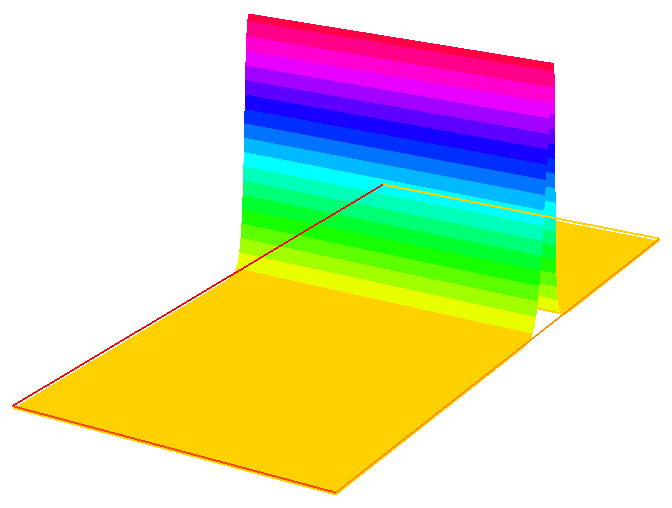
\includegraphics[scale=0.3]{images/capture1.png}
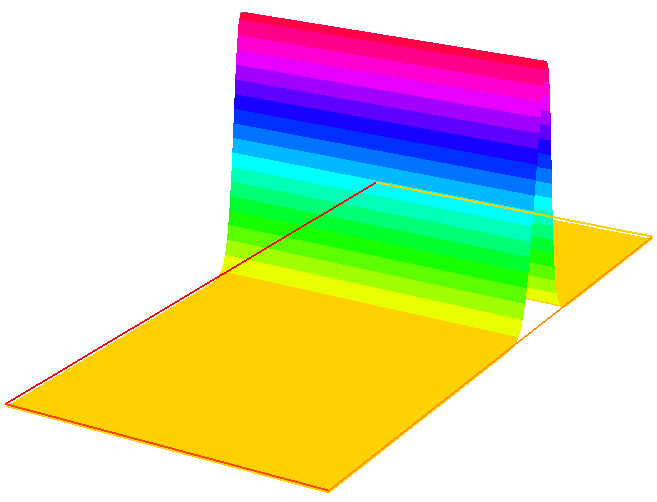
\includegraphics[scale=0.3]{images/capture2.png}\\
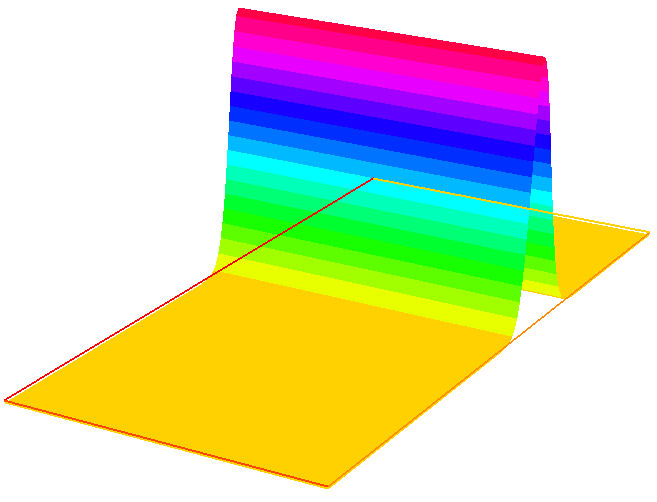
\includegraphics[scale=0.3]{images/capture3.png}
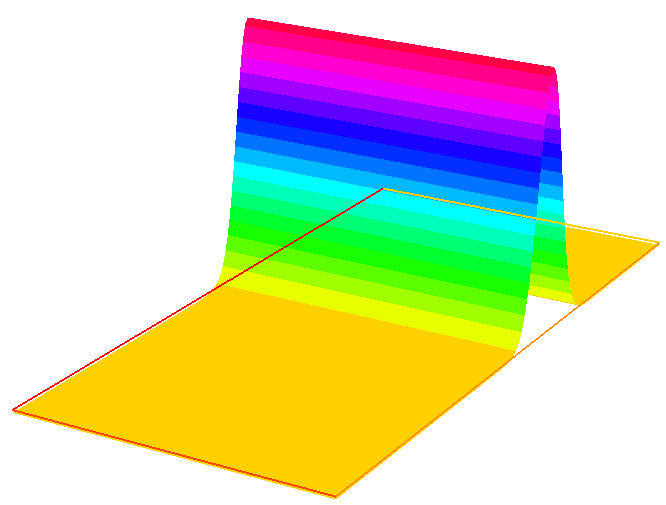
\includegraphics[scale=0.3]{images/capture4.png}\\
\begin{figure}[!h]
\begin{center}
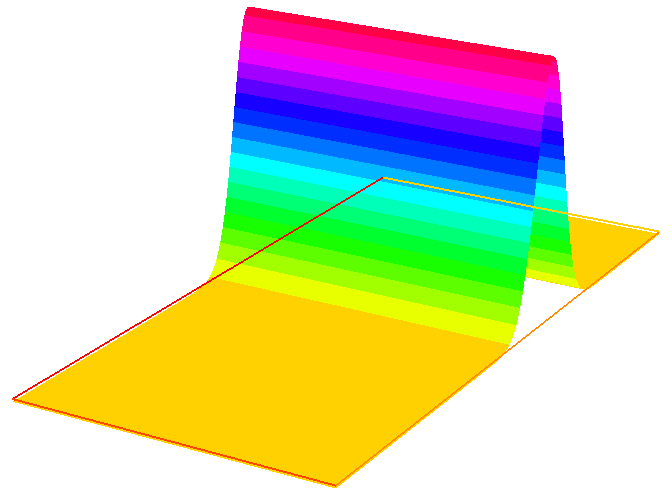
\includegraphics[scale=0.3]{images/capture5.png}
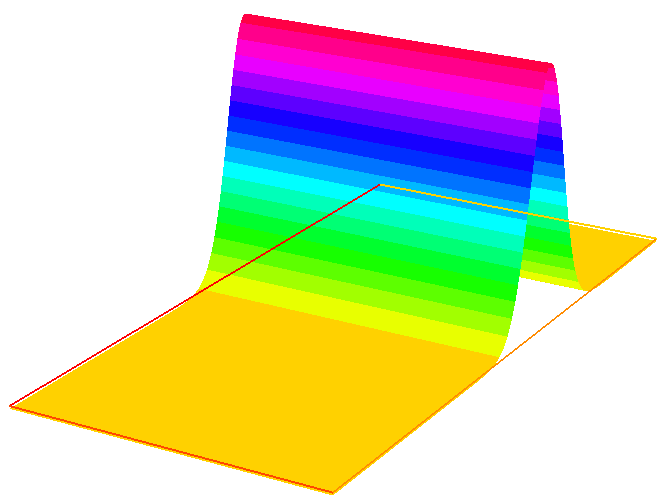
\includegraphics[scale=0.3]{images/capture6.png}\\
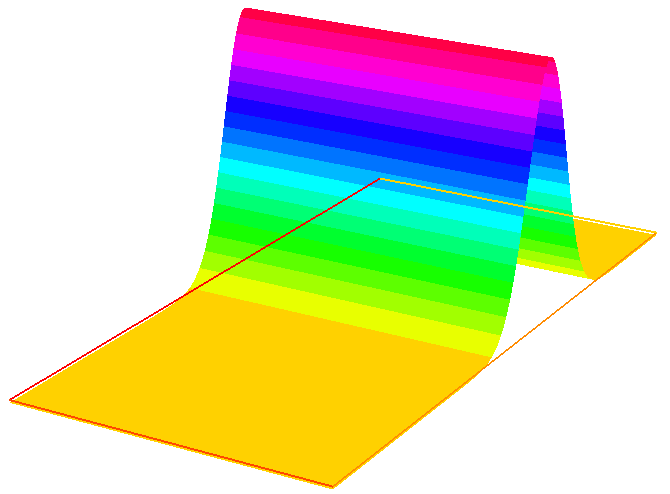
\includegraphics[scale=0.3]{images/capture7.png}
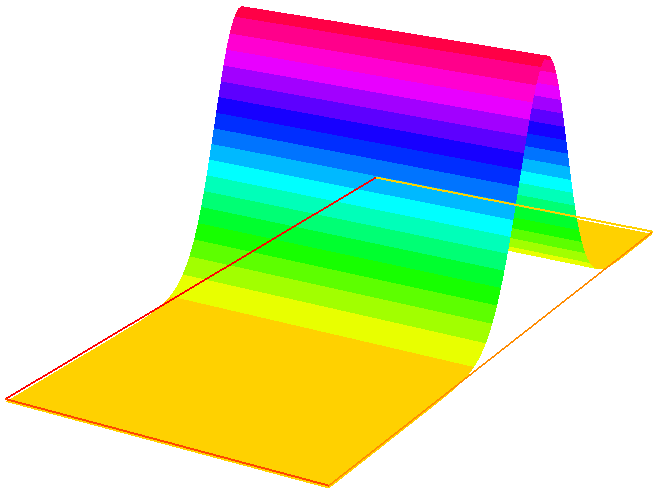
\includegraphics[scale=0.3]{images/capture8.png}
\end{center}
\caption{Captures d'écran obtenus par le logiciel FreeFem++ à différents moments}
\label{freeFemSV}
\end{figure}
